\documentclass{ximera}

\usepackage{epsfig}

\graphicspath{
  {./}
  {figures/}
}

\usepackage{epstopdf}
%\usepackage{ulem}
\usepackage[normalem]{ulem}

\epstopdfsetup{outdir=./}

\usepackage{morewrites}
\makeatletter
\newcommand\subfile[1]{%
\renewcommand{\input}[1]{}%
\begingroup\skip@preamble\otherinput{#1}\endgroup\par\vspace{\topsep}
\let\input\otherinput}
\makeatother

\newcommand{\EXER}{}
\newcommand{\includeexercises}{\EXER\directlua{dofile(kpse.find_file("exercises","lua"))}}

\newenvironment{computerExercise}{\begin{exercise}}{\end{exercise}}

%\newcounter{ccounter}
%\setcounter{ccounter}{1}
%\newcommand{\Chapter}[1]{\setcounter{chapter}{\arabic{ccounter}}\chapter{#1}\addtocounter{ccounter}{1}}

%\newcommand{\section}[1]{\section{#1}\setcounter{thm}{0}\setcounter{equation}{0}}

%\renewcommand{\theequation}{\arabic{chapter}.\arabic{section}.\arabic{equation}}
%\renewcommand{\thefigure}{\arabic{chapter}.\arabic{figure}}
%\renewcommand{\thetable}{\arabic{chapter}.\arabic{table}}

%\newcommand{\Sec}[2]{\section{#1}\markright{\arabic{ccounter}.\arabic{section}.#2}\setcounter{equation}{0}\setcounter{thm}{0}\setcounter{figure}{0}}
  
\newcommand{\Sec}[2]{\section{#1}}

\setcounter{secnumdepth}{2}
%\setcounter{secnumdepth}{1} 

%\newcounter{THM}
%\renewcommand{\theTHM}{\arabic{chapter}.\arabic{section}}

\newcommand{\trademark}{{R\!\!\!\!\!\bigcirc}}
%\newtheorem{exercise}{}

\newcommand{\dfield}{{\sf SlopeField}}

\newcommand{\pplane}{{\sf PhasePlane}}

\newcommand{\PPLANE}{{\sf PHASEPLANE}}

% BADBAD: \newcommand{\Bbb}{\bf}. % Package amsfonts Warning: Obsolete command \Bbb; \mathbb should be used instead.

\newcommand{\R}{\mbox{$\mathbb{R}$}}
\let\C\relax
\newcommand{\C}{\mbox{$\mathbb{C}$}}
\newcommand{\Z}{\mbox{$\mathbb{Z}$}}
\newcommand{\N}{\mbox{$\mathbb{N}$}}
\newcommand{\D}{\mbox{{\bf D}}}

\newcommand{\WW}{\mathcal{W}}

\usepackage{amssymb}
%\newcommand{\qed}{\hfill\mbox{\raggedright$\square$} \vspace{1ex}}
%\newcommand{\proof}{\noindent {\bf Proof:} \hspace{0.1in}}

\newcommand{\setmin}{\;\mbox{--}\;}
\newcommand{\Matlab}{{M\small{AT\-LAB}} }
\newcommand{\Matlabp}{{M\small{AT\-LAB}}}
\newcommand{\computer}{\Matlab Instructions}
\renewcommand{\computer}{M\small{ATLAB} Instructions}
\newcommand{\half}{\mbox{$\frac{1}{2}$}}
\newcommand{\compose}{\raisebox{.15ex}{\mbox{{\scriptsize$\circ$}}}}
\newcommand{\AND}{\quad\mbox{and}\quad}
\newcommand{\vect}[2]{\left(\begin{array}{c} #1_1 \\ \vdots \\
 #1_{#2}\end{array}\right)}
\newcommand{\mattwo}[4]{\left(\begin{array}{rr} #1 & #2\\ #3
&#4\end{array}\right)}
\newcommand{\mattwoc}[4]{\left(\begin{array}{cc} #1 & #2\\ #3
&#4\end{array}\right)}
\newcommand{\vectwo}[2]{\left(\begin{array}{r} #1 \\ #2\end{array}\right)}
\newcommand{\vectwoc}[2]{\left(\begin{array}{c} #1 \\ #2\end{array}\right)}

\newcommand{\ignore}[1]{}


\newcommand{\inv}{^{-1}}
\newcommand{\CC}{{\cal C}}
\newcommand{\CCone}{\CC^1}
\newcommand{\Span}{{\rm span}}
\newcommand{\rank}{{\rm rank}}
\newcommand{\trace}{{\rm tr}}
\newcommand{\RE}{{\rm Re}}
\newcommand{\IM}{{\rm Im}}
\newcommand{\nulls}{{\rm null\;space}}

\newcommand{\dps}{\displaystyle}
\newcommand{\arraystart}{\renewcommand{\arraystretch}{1.8}}
\newcommand{\arrayfinish}{\renewcommand{\arraystretch}{1.2}}
\newcommand{\Start}[1]{\vspace{0.08in}\noindent {\bf Section~\ref{#1}}}
\newcommand{\exer}[1]{\noindent {\bf \ref{#1}}}
\newcommand{\ans}{\textbf{Answer:} }
\newcommand{\matthree}[9]{\left(\begin{array}{rrr} #1 & #2 & #3 \\ #4 & #5 & #6
\\ #7 & #8 & #9\end{array}\right)}
\newcommand{\cvectwo}[2]{\left(\begin{array}{c} #1 \\ #2\end{array}\right)}
\newcommand{\cmatthree}[9]{\left(\begin{array}{ccc} #1 & #2 & #3 \\ #4 & #5 &
#6 \\ #7 & #8 & #9\end{array}\right)}
\newcommand{\vecthree}[3]{\left(\begin{array}{r} #1 \\ #2 \\
#3\end{array}\right)}
\newcommand{\cvecthree}[3]{\left(\begin{array}{c} #1 \\ #2 \\
#3\end{array}\right)}
\newcommand{\cmattwo}[4]{\left(\begin{array}{cc} #1 & #2\\ #3
&#4\end{array}\right)}

\newcommand{\Matrix}[1]{\ensuremath{\left(\begin{array}{rrrrrrrrrrrrrrrrrr} #1 \end{array}\right)}}

\newcommand{\Matrixc}[1]{\ensuremath{\left(\begin{array}{cccccccccccc} #1 \end{array}\right)}}



\renewcommand{\labelenumi}{\theenumi}
\newenvironment{enumeratea}%
{\begingroup
 \renewcommand{\theenumi}{\alph{enumi}}
 \renewcommand{\labelenumi}{(\theenumi)}
 \begin{enumerate}}
 {\end{enumerate}
 \endgroup}

\newcounter{help}
\renewcommand{\thehelp}{\thesection.\arabic{equation}}

%\newenvironment{equation*}%
%{\renewcommand\endequation{\eqno (\theequation)* $$}%
%   \begin{equation}}%
%   {\end{equation}\renewcommand\endequation{\eqno \@eqnnum
%$$\global\@ignoretrue}}

%\input{psfig.tex}

\author{Martin Golubitsky and Michael Dellnitz}

%\newenvironment{matlabEquation}%
%{\renewcommand\endequation{\eqno (\theequation*) $$}%
%   \begin{equation}}%
%   {\end{equation}\renewcommand\endequation{\eqno \@eqnnum
% $$\global\@ignoretrue}}

\newcommand{\soln}{\textbf{Solution:} }
\newcommand{\exercap}[1]{\centerline{Figure~\ref{#1}}}
\newcommand{\exercaptwo}[1]{\centerline{Figure~\ref{#1}a\hspace{2.1in}
Figure~\ref{#1}b}}
\newcommand{\exercapthree}[1]{\centerline{Figure~\ref{#1}a\hspace{1.2in}
Figure~\ref{#1}b\hspace{1.2in}Figure~\ref{#1}c}}
\newcommand{\para}{\hspace{0.4in}}

\usepackage{ifluatex}
\ifluatex
\ifcsname displaysolutions\endcsname%
\else
\renewenvironment{solution}{\suppress}{\endsuppress}
\fi
\else
\renewenvironment{solution}{}{}
\fi

\ifcsname answer\endcsname
\renewcommand{\answer}{}
\fi

%\ifxake
%\newenvironment{matlabEquation}{\begin{equation}}{\end{equation}}
%\else
\newenvironment{matlabEquation}%
{\let\oldtheequation\theequation\renewcommand{\theequation}{\oldtheequation*}\begin{equation}}%
  {\end{equation}\let\theequation\oldtheequation}
%\fi

\makeatother

\newcommand{\RED}[1]{{\color{red}{#1}}} 


\title{Two Species Population Models}

\begin{document}
\begin{abstract}
\end{abstract}
\maketitle


\label{S:TSPM} \index{population model}

Suppose that two species coexist in an isolated environment and
that we want to understand how the populations of both species
evolve in time.  Denote the population of the first species at time 
$t$ by $x(t)\ge 0$ and the population of the second species
by $y(t)\ge 0$.  There is one general assumption about models of
population growth that we make: If at any time $t$ the
population of a species is zero (that is, the population is {\em
extinct\/}), then the population of that species is zero for all
subsequent time.  In short, extinct populations remain extinct.

If the evolution of the population of two species is modeled by a
first order system of autonomous equations, then the model has the form
\begin{eqnarray}
\frac{dx}{dt} & = & xf_1(x,y) \label{e:pop1a} \\
\frac{dy}{dt} & = & yf_2(x,y) \label{e:pop1b}
\end{eqnarray}  \index{population model!two species}
where $x,y \ge 0$.
The presence of the factor $x$ in \eqref{e:pop1a} and the factor
$y$ in \eqref{e:pop1b} insures that extinct populations remain
extinct. The factors $f_j$ are the {\em growth rates\/} of the 
species.\index{growth rate}

If $f_1(x,y) = \mu_1$ and $f_2(x,y)=\mu_2$ are constants, then 
the system \eqref{e:pop1a},\eqref{e:pop1b} is an uncoupled system 
of linear equations, and the two species evolve independently.  
In this model, the population of species $j$ either grows
exponentially ($\mu_j>0$) or decays exponentially ($\mu_j<0$)
or remains constant ($\mu_j=0$).


\subsection*{Predator-Prey Equations}
\index{predator-prey equation}

Several assumptions go into the development of predator-prey 
models. 
\begin{itemize}
\item[(a)]  In the absence of predators, the prey population
grows.
\item[(b)]  In the absence of prey, the predator population 
shrinks.
\item[(c)]  In the presence of predators, the growth rate of
the prey population decreases.
\item[(d)]  In the presence of prey, the growth rate of the 
predator population increases.
\end{itemize}
Let $x$ denote the size of the prey population
\index{prey population} and $y$ denote 
the size of the predator population\index{predator population}.  
The simplest model that 
incorporates these four assumptions is:
\begin{matlabEquation} \label{e:PP}
\begin{array}{lcr}
\dot{x} & = & x(\mu_1 + \sigma_1y)\; \\
\dot{y} & = & y(\mu_2 + \sigma_2x),
\end{array}
\end{matlabEquation}\index{predator-prey equation}
where $\mu_1,\mu_2,\sigma_1,\sigma_2$ are constants.  Assumptions
(a)--(d) can be restated simply as 
\begin{itemize}
\item[(a)]  $\mu_1 > 0$.
\item[(b)]  $\mu_2 < 0$.
\item[(c)]  $\sigma_1 < 0$.
\item[(d)]  $\sigma_2 > 0$.
\end{itemize}
  
Under these assumptions, what can we expect the fate of predator-prey 
populations to be?  Remarkably, most solutions to the differential equations 
\eqref{e:PP} are periodic solutions\index{periodic solution}.  
We test this statement using 
{\pplane}\index{\computer!pplane8}.   
Loading system {\tt e12\_1\_3.pps} into {\pplane}
we find the predator-prey equations with default values
\[
\mu_1 = 0.4, \quad \mu_2 = -0.3, \quad \sigma_1 = -0.01, \quad \sigma_2 = 0.005.
\]
Press the {\sf Proceed} button and plot several trajectories.  You
should find a picture like that in Figure~\ref{F:PP1}.  In this figure 
there is an equilibrium at $(x,y)=(60,40)$ surrounded by periodic 
trajectories. 

\begin{figure}[htb]
           \centerline{%
	   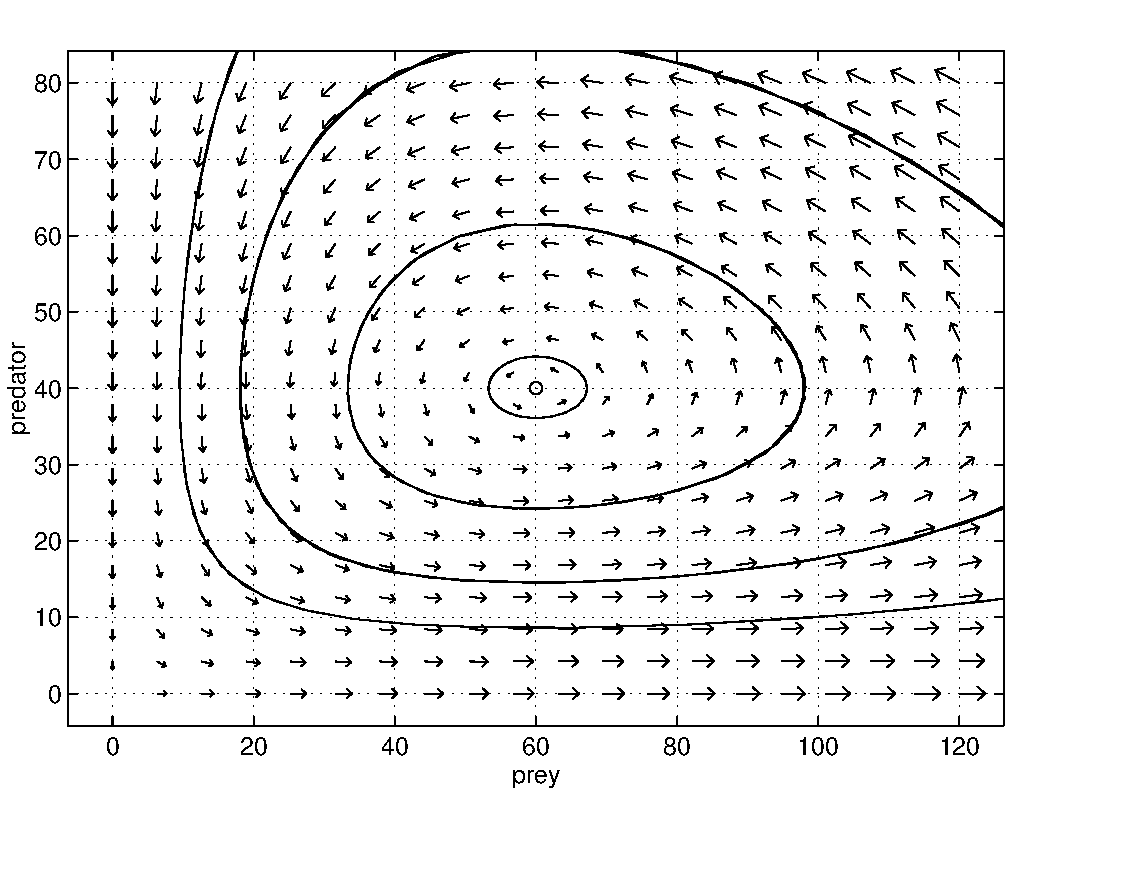
\includegraphics[height=3.0in]{../figures/pp1.pdf}}
           \caption{Phase portrait for predator-prey equations 
		\protect\eqref{e:PP}.}
           \label{F:PP1}
\end{figure}

Note that if a solution to the predator-prey equation is time periodic, then 
the predator population and the prey population both vary periodically with 
the same period.  The assumptions (a)--(d) that went into forming the
predator-prey equations \eqref{e:PP} are reflected in the time periodic 
solutions drawn in Figure~\ref{F:PP1}.  To see this correspondence, note that 
when the predator and the prey populations are near their minimum values, then 
the prey population increases while the predator population remains nearly 
constant (assumption (a)).  After awhile, however, first the predator growth
rate and then the predator population increase (assumption (d)), and the prey 
population begins to fall (assumption (c)).  Then the prey population falls 
further and, as it does, the predator growth rate decreases (assumption (b)). 
Finally, the predator population falls until both populations are near their 
minimum values, and the whole process repeats itself exactly --- at least in
this model.  

\subsubsection*{Scaling and Reduction in the Number of Parameters}

From the discussion in Chapter~\ref{C:NPS} on Morse-Smale differential
equations, it should seem surprising that a system of nonlinear differential 
equations produces an equilibrium surrounded by a continuous family of 
periodic solutions --- just as the linear center does. \index{center} You 
might think that the values of the constants $\mu_1,\mu_2,\sigma_1,\sigma_2$ 
were chosen just so this unlikely situation would occur.  In fact, this is 
not the case as a little numerical experimentation with different values of 
$\mu_1,\mu_2,\sigma_1,\sigma_2$ will show.  

It is also surprising that a differential equation depending on four
parameters would have similar phase portraits for every one of
these parameters (assuming the appropriate sign restrictions on
the parameters).  We continue our discussion of \eqref{e:PP} by using scaling
arguments to show that three of these parameters are inessential.  

The idea behind scaling is simple.  We think of $x(t)$ as measuring the 
number of some species at time $t$.  But what is the measure?  Are we 
counting the number of individuals or the number of thousands of
individuals or even the number of millions of individuals?  For example, 
we say that the population of the United States is 275 
million people.  Similarly, when speaking of population growth, 
we choose a time unit.  Is population growth measured per year 
or per month or, in the case of bacteria, per minute?  In general, we can 
change the units of population and time without changing the type of 
solutions.  We make this change in scale by setting \index{scaling} 
\[
X(t) = \alpha x(\gamma t)  \AND  Y(t) = \beta y(\gamma t),
\]
where $\alpha,\beta,\gamma$ are positive scaling constants.  

Next, we derive differential equations for $X$ and $Y$ using the
chain rule\index{chain rule} and the differential 
equations \eqref{e:PP}. Observe that 
\[
\frac{dX}{dt}(t) = \alpha \gamma \frac{dx}{dt}(\gamma t) \AND  
\frac{dY}{dt}(t) = \beta \gamma \frac{dy}{dt}(\gamma t),
\]
and from \eqref{e:PP} that 
\begin{eqnarray*}
\frac{dX}{dt}(t) & = & \alpha \gamma \frac{dx}{dt}(\gamma t) \\
& = & \alpha \gamma x(\gamma t)(\mu_1 + \sigma_1y(\gamma t)) \\
& = & \gamma X(t)(\mu_1 + \frac{\sigma_1}{\beta}Y(t)).
\end{eqnarray*}
A similar equation holds for $\dot{Y}$.  Dropping the explicit 
dependence on $t$, we have
\begin{eqnarray*}
\frac{dX}{dt} & = & X(\gamma \mu_1 + \frac{\gamma\sigma_1}{\beta}Y)\\
\frac{dY}{dt} & = & Y(\gamma \mu_2 + \frac{\gamma\sigma_2}{\alpha}X).
\end{eqnarray*}
We now make a judicious choice of the three constants $\alpha,\beta,
\gamma$.  We choose
\begin{equation}  \label{E:scalingcoeff}
\alpha = \gamma\sigma_2, \quad \beta = -\gamma\sigma_1, \AND
\gamma = -\frac{1}{\mu_2}.
\end{equation}
These choices lead to the system of differential equations
\begin{matlabEquation}  \label{e:PP2}
\begin{array}{lcl}
\dot{X} & = & X(\mu - Y) \\
\dot{Y} & = & Y(-1 + X),
\end{array}
\end{matlabEquation}% \index{predator-prey equation}
where $\mu = \left|\frac{\mu_1}{\mu_2}\right|>0$.  It is easy to 
check that the scaled predator-prey equations \eqref{e:PP2} have 
an equilibrium at $(X,Y)=(1,\mu)$ that is a center.  It is also 
easy to check using {\pplane} that for each $\mu$ the phase 
portrait of \eqref{e:PP2} appears to have periodic solutions 
surrounding this center.

\subsection*{The Volterra-Lotka Equations}
\index{Volterra-Lotka equations}

Next we show that if the population model \eqref{e:PP} is extended to 
a more complicated model, then the family of periodic 
solutions\index{family of periodic solutions} in 
the predator-prey equations disappears.  To understand better the 
extension that we have in mind for the predator-prey equations, we 
discuss first the single species logistic equation.
 
The {\em logistic equation\/} \index{logistic equation} is:
\[
\frac{dx}{dt} = x(\mu_1 + \rho_1x).
\]
In this model the growth rate of the population is assumed to
depend on the size of the population.  Typically, it is assumed
that the growth rate decreases as the population increases; that
is, it is assumed that $\rho_1 < 0$.  It follows that the
logistic model for two independent species is the uncoupled system:
\begin{eqnarray*}
\dot{x} & = & x(\mu_1 + \rho_1x) \\
\dot{y} & = & y(\mu_2 + \rho_2y),
\end{eqnarray*}
where $\mu_j>0,\rho_j<0$.

The {\em Volterra-Lotka\/} equations\index{Volterra-Lotka equations} 
are the simplest extension
of the uncoupled logistic system to interacting species, and
have the form:
\begin{equation} \label{e:pop2}
\begin{array}{rcl}
\dot{x} & = & x(\mu_1 +   \rho_1x + \sigma_1y) \\
\dot{y} & = & y(\mu_2 + \sigma_2x +   \rho_2y),
\end{array}
\end{equation}
where $\sigma_1,\sigma_2$ are nonzero constants.  Note that when
$\sigma_1=\sigma_2=0$ system \eqref{e:pop2} reduces to the
uncoupled logistic system. 

These equations model three different types of situations.  If
$\sigma_1>0$, then the population growth rate of the first species 
increases as the population of the second species increases.  If
$\sigma_2<0$, the population growth rate of the second species
slows as the population of the first species increases.
Suppose that the signs of $\sigma_1$ and $\sigma_2$ are
different, that is, suppose $\sigma_1<0$ and $\sigma_2>0$.  Then
the second species acts like predators (the more of the second
species there is, the lower the growth rate of the first
species), and the first species acts like prey (the more of
the first species there is, the higher the growth rate of the
second species).  In this case, the Volterra-Lotka equations are
a generalized predator-prey two species model.  Indeed,
if $\rho_1=\rho_2=0$ in \eqref{e:pop2}, then we recover the
predator-prey equations \eqref{e:PP}.  Thus, we may think of
Volterra-Lotka equations as a small perturbation of the 
predator-prey equations when $\rho_1$ and $\rho_2$ are small.
The two other cases in \eqref{e:pop2} correspond to {\em competing\/} 
species\index{competing species} ($\sigma_1,\sigma_2<0$) and 
{\em cooperating\/} species\index{cooperating species}
($\sigma_1,\sigma_2>0$).


\subsubsection*{Predator-Prey Volterra-Lotka Equations}
\index{predator-prey equation}\index{Volterra-Lotka equations}

What kind of population dynamics are predicted by equations
\eqref{e:pop2}?  The answer depends on the exact values of the 
six parameters $\mu_j,\rho_j,\sigma_j$.  As in our previous
discussion of the predator-prey equations \eqref{e:PP}, we assume
that $\mu_1>0$ and $\mu_2<0$.  To simplify the notation, we
perform the same scalings as we did when transforming \eqref{e:PP} 
to \eqref{e:PP2}, and obtain
\begin{eqnarray*} 
\dot{x} & = & x(\mu + \rho x -       y) \\
\dot{y} & = & y( -1 +       x + \eta y),
\end{eqnarray*}
where $\mu>0,\rho,\eta$ are constants.  \index{predator-prey equation}

We wish to compare the dynamics of these equations with those of 
the predator-prey model \eqref{e:PP}. To facilitate this 
comparison, we assume that $\eta=0$ and study the system of 
equations
\begin{matlabEquation} \label{e:pop3}
\begin{array}{rcl}
\dot{x} & = & x(\mu + \rho x -       y) \\
\dot{y} & = & y( -1 +       x).
\end{array}
\end{matlabEquation}
There is one equilibrium\index{equilibrium} where neither species 
is extinct
(that is, where $x>0$ and $y>0$).  For population dynamics the 
equilibrium $(x,y)=(1,\mu+\rho)$ is a relevant solution to 
\eqref{e:pop3} only when $\mu+\rho>0$, as we care about solutions only 
when $x\geq0, y\geq 0$.  To understand the dynamics near this
equilibrium, we compute the Jacobian matrix
\[
\mattwoc{\mu + 2\rho x-y }{-x}{y}{-1+x} = 
\mattwoc{\rho}{-1}{\mu+\rho}{0}.
\]
The determinant\index{determinant} of this matrix is $\mu+\rho>0$ and 
the trace\index{trace} is $\rho$.  Fix $\mu>0$.   It follows that for 
$\rho$ near zero and negative this equilibrium is a spiral 
sink\index{sink} and for $\rho$ near zero and positive this 
equilibrium is a spiral source\index{source}.  The
phase portraits\index{phase!portrait} for these two cases are shown in
Figure~\ref{F:pop3}.  So we see that as long as $\rho\neq 0$,
the continuous family of periodic solutions found in the simpler
predator-prey equations \eqref{e:PP} disappears.\index{periodic solution}


\begin{figure*}[htb]
           \centerline{%
	   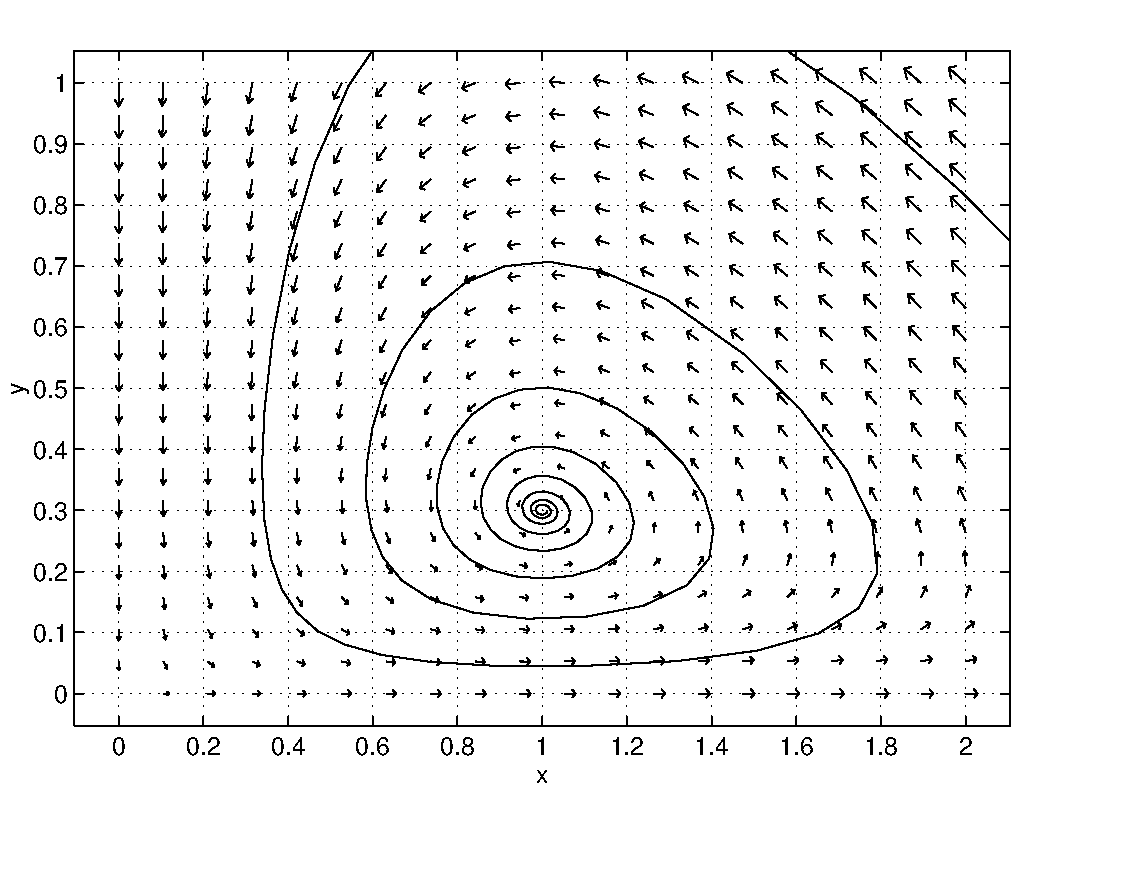
\includegraphics[height=2.5in]{../figures/pop3a.pdf}
	   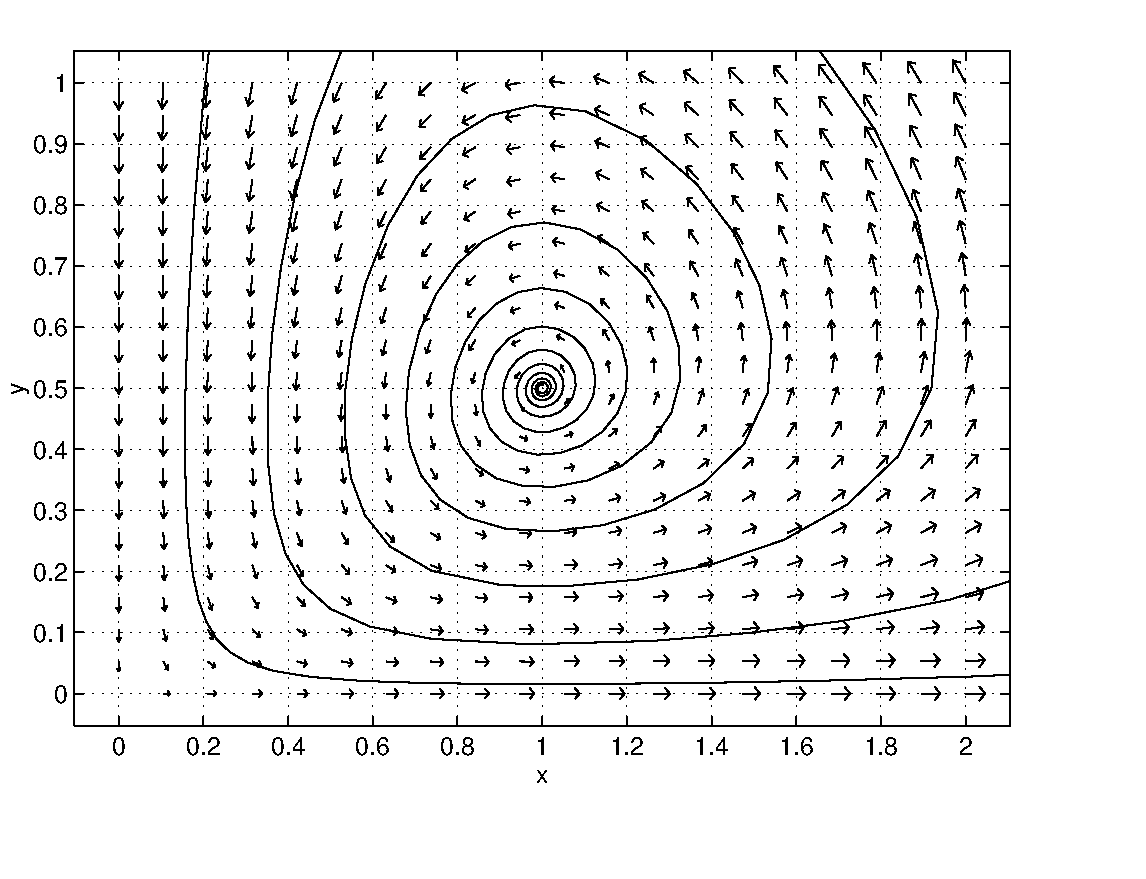
\includegraphics[height=2.5in]{../figures/pop3b.pdf}}
		\vspace*{-0.2in}		
		\hspace{1.0in} $\rho=-0.1$ \hspace{2.5in} $\rho=0.1$
           \caption{Phase portraits for Volterra-Lotka predator-prey 
		equations \protect\eqref{e:pop3} with $\mu=0.4$.}
           \label{F:pop3}
\end{figure*}



\includeexercises


\end{document}
